% Created by tikzDevice version 0.12.6 on 2025-02-14 16:42:54
% !TEX encoding = UTF-8 Unicode
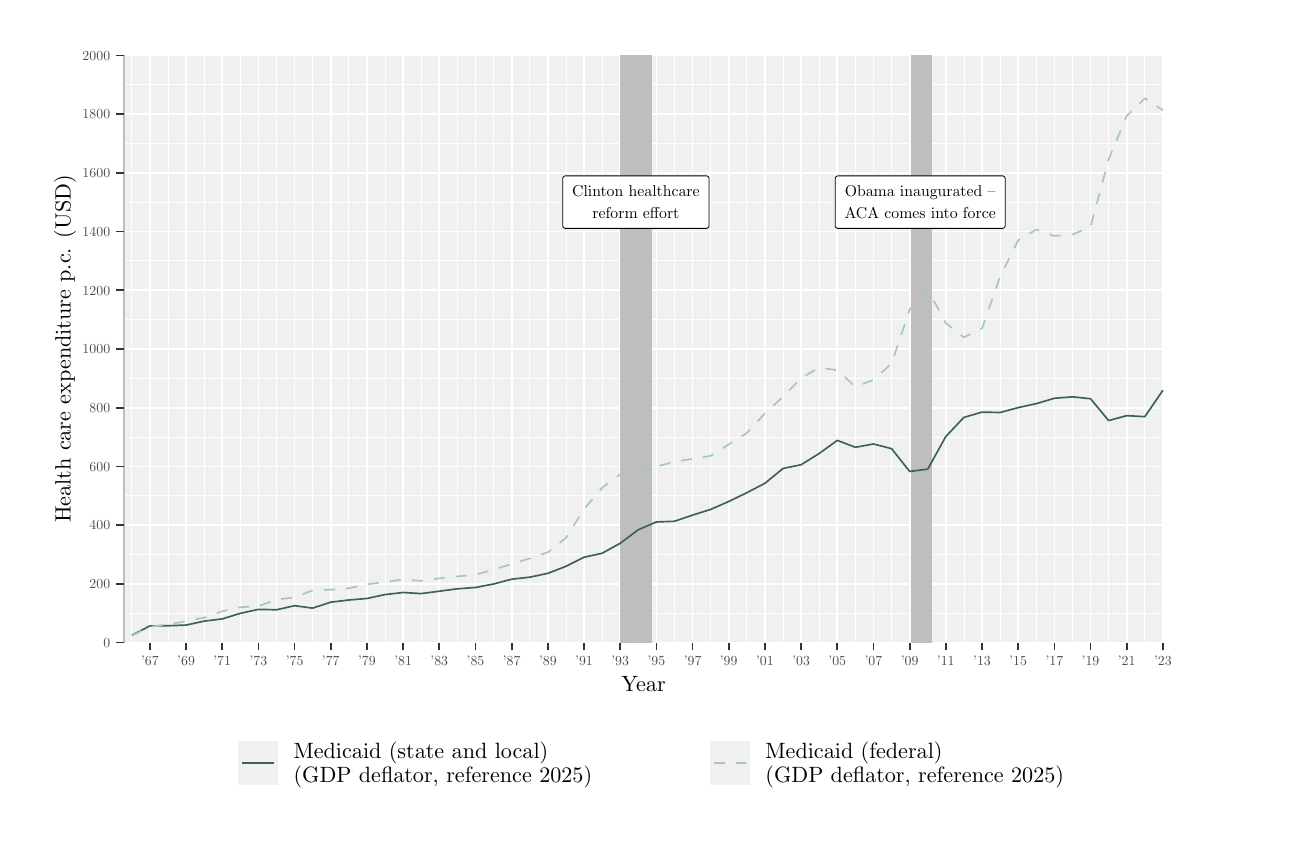
\begin{tikzpicture}[x=1pt,y=1pt]
\definecolor{fillColor}{RGB}{255,255,255}
\path[use as bounding box,fill=fillColor,fill opacity=0.00] (0,0) rectangle (455.30,289.08);
\begin{scope}
\path[clip] (  0.00,  0.00) rectangle (455.30,289.08);
\definecolor{drawColor}{RGB}{255,255,255}
\definecolor{fillColor}{RGB}{255,255,255}

\path[draw=drawColor,line width= 0.6pt,line join=round,line cap=round,fill=fillColor] ( -0.00,  0.00) rectangle (455.30,289.08);
\end{scope}
\begin{scope}
\path[clip] (  0.00,  0.00) rectangle (455.30,289.08);
\definecolor{fillColor}{gray}{0.94}

\path[fill=fillColor] ( 34.76, 66.89) rectangle (410.30,279.08);
\definecolor{drawColor}{RGB}{255,255,255}

\path[draw=drawColor,line width= 0.3pt,line join=round] ( 34.76, 77.50) --
	(410.30, 77.50);

\path[draw=drawColor,line width= 0.3pt,line join=round] ( 34.76, 98.71) --
	(410.30, 98.71);

\path[draw=drawColor,line width= 0.3pt,line join=round] ( 34.76,119.93) --
	(410.30,119.93);

\path[draw=drawColor,line width= 0.3pt,line join=round] ( 34.76,141.15) --
	(410.30,141.15);

\path[draw=drawColor,line width= 0.3pt,line join=round] ( 34.76,162.37) --
	(410.30,162.37);

\path[draw=drawColor,line width= 0.3pt,line join=round] ( 34.76,183.59) --
	(410.30,183.59);

\path[draw=drawColor,line width= 0.3pt,line join=round] ( 34.76,204.81) --
	(410.30,204.81);

\path[draw=drawColor,line width= 0.3pt,line join=round] ( 34.76,226.03) --
	(410.30,226.03);

\path[draw=drawColor,line width= 0.3pt,line join=round] ( 34.76,247.25) --
	(410.30,247.25);

\path[draw=drawColor,line width= 0.3pt,line join=round] ( 34.76,268.47) --
	(410.30,268.47);

\path[draw=drawColor,line width= 0.3pt,line join=round] ( 37.63, 66.89) --
	( 37.63,279.08);

\path[draw=drawColor,line width= 0.3pt,line join=round] ( 50.70, 66.89) --
	( 50.70,279.08);

\path[draw=drawColor,line width= 0.3pt,line join=round] ( 63.77, 66.89) --
	( 63.77,279.08);

\path[draw=drawColor,line width= 0.3pt,line join=round] ( 76.85, 66.89) --
	( 76.85,279.08);

\path[draw=drawColor,line width= 0.3pt,line join=round] ( 89.92, 66.89) --
	( 89.92,279.08);

\path[draw=drawColor,line width= 0.3pt,line join=round] (102.99, 66.89) --
	(102.99,279.08);

\path[draw=drawColor,line width= 0.3pt,line join=round] (116.07, 66.89) --
	(116.07,279.08);

\path[draw=drawColor,line width= 0.3pt,line join=round] (129.14, 66.89) --
	(129.14,279.08);

\path[draw=drawColor,line width= 0.3pt,line join=round] (142.21, 66.89) --
	(142.21,279.08);

\path[draw=drawColor,line width= 0.3pt,line join=round] (155.29, 66.89) --
	(155.29,279.08);

\path[draw=drawColor,line width= 0.3pt,line join=round] (168.36, 66.89) --
	(168.36,279.08);

\path[draw=drawColor,line width= 0.3pt,line join=round] (181.43, 66.89) --
	(181.43,279.08);

\path[draw=drawColor,line width= 0.3pt,line join=round] (194.51, 66.89) --
	(194.51,279.08);

\path[draw=drawColor,line width= 0.3pt,line join=round] (207.58, 66.89) --
	(207.58,279.08);

\path[draw=drawColor,line width= 0.3pt,line join=round] (220.65, 66.89) --
	(220.65,279.08);

\path[draw=drawColor,line width= 0.3pt,line join=round] (233.73, 66.89) --
	(233.73,279.08);

\path[draw=drawColor,line width= 0.3pt,line join=round] (246.80, 66.89) --
	(246.80,279.08);

\path[draw=drawColor,line width= 0.3pt,line join=round] (259.87, 66.89) --
	(259.87,279.08);

\path[draw=drawColor,line width= 0.3pt,line join=round] (272.95, 66.89) --
	(272.95,279.08);

\path[draw=drawColor,line width= 0.3pt,line join=round] (286.02, 66.89) --
	(286.02,279.08);

\path[draw=drawColor,line width= 0.3pt,line join=round] (299.09, 66.89) --
	(299.09,279.08);

\path[draw=drawColor,line width= 0.3pt,line join=round] (312.17, 66.89) --
	(312.17,279.08);

\path[draw=drawColor,line width= 0.3pt,line join=round] (325.24, 66.89) --
	(325.24,279.08);

\path[draw=drawColor,line width= 0.3pt,line join=round] (338.31, 66.89) --
	(338.31,279.08);

\path[draw=drawColor,line width= 0.3pt,line join=round] (351.39, 66.89) --
	(351.39,279.08);

\path[draw=drawColor,line width= 0.3pt,line join=round] (364.46, 66.89) --
	(364.46,279.08);

\path[draw=drawColor,line width= 0.3pt,line join=round] (377.53, 66.89) --
	(377.53,279.08);

\path[draw=drawColor,line width= 0.3pt,line join=round] (390.61, 66.89) --
	(390.61,279.08);

\path[draw=drawColor,line width= 0.3pt,line join=round] (403.68, 66.89) --
	(403.68,279.08);

\path[draw=drawColor,line width= 0.6pt,line join=round] ( 34.76, 66.89) --
	(410.30, 66.89);

\path[draw=drawColor,line width= 0.6pt,line join=round] ( 34.76, 88.10) --
	(410.30, 88.10);

\path[draw=drawColor,line width= 0.6pt,line join=round] ( 34.76,109.32) --
	(410.30,109.32);

\path[draw=drawColor,line width= 0.6pt,line join=round] ( 34.76,130.54) --
	(410.30,130.54);

\path[draw=drawColor,line width= 0.6pt,line join=round] ( 34.76,151.76) --
	(410.30,151.76);

\path[draw=drawColor,line width= 0.6pt,line join=round] ( 34.76,172.98) --
	(410.30,172.98);

\path[draw=drawColor,line width= 0.6pt,line join=round] ( 34.76,194.20) --
	(410.30,194.20);

\path[draw=drawColor,line width= 0.6pt,line join=round] ( 34.76,215.42) --
	(410.30,215.42);

\path[draw=drawColor,line width= 0.6pt,line join=round] ( 34.76,236.64) --
	(410.30,236.64);

\path[draw=drawColor,line width= 0.6pt,line join=round] ( 34.76,257.86) --
	(410.30,257.86);

\path[draw=drawColor,line width= 0.6pt,line join=round] ( 34.76,279.08) --
	(410.30,279.08);

\path[draw=drawColor,line width= 0.6pt,line join=round] ( 44.16, 66.89) --
	( 44.16,279.08);

\path[draw=drawColor,line width= 0.6pt,line join=round] ( 57.24, 66.89) --
	( 57.24,279.08);

\path[draw=drawColor,line width= 0.6pt,line join=round] ( 70.30, 66.89) --
	( 70.30,279.08);

\path[draw=drawColor,line width= 0.6pt,line join=round] ( 83.39, 66.89) --
	( 83.39,279.08);

\path[draw=drawColor,line width= 0.6pt,line join=round] ( 96.45, 66.89) --
	( 96.45,279.08);

\path[draw=drawColor,line width= 0.6pt,line join=round] (109.53, 66.89) --
	(109.53,279.08);

\path[draw=drawColor,line width= 0.6pt,line join=round] (122.60, 66.89) --
	(122.60,279.08);

\path[draw=drawColor,line width= 0.6pt,line join=round] (135.68, 66.89) --
	(135.68,279.08);

\path[draw=drawColor,line width= 0.6pt,line join=round] (148.74, 66.89) --
	(148.74,279.08);

\path[draw=drawColor,line width= 0.6pt,line join=round] (161.83, 66.89) --
	(161.83,279.08);

\path[draw=drawColor,line width= 0.6pt,line join=round] (174.89, 66.89) --
	(174.89,279.08);

\path[draw=drawColor,line width= 0.6pt,line join=round] (187.97, 66.89) --
	(187.97,279.08);

\path[draw=drawColor,line width= 0.6pt,line join=round] (201.04, 66.89) --
	(201.04,279.08);

\path[draw=drawColor,line width= 0.6pt,line join=round] (214.12, 66.89) --
	(214.12,279.08);

\path[draw=drawColor,line width= 0.6pt,line join=round] (227.18, 66.89) --
	(227.18,279.08);

\path[draw=drawColor,line width= 0.6pt,line join=round] (240.27, 66.89) --
	(240.27,279.08);

\path[draw=drawColor,line width= 0.6pt,line join=round] (253.33, 66.89) --
	(253.33,279.08);

\path[draw=drawColor,line width= 0.6pt,line join=round] (266.41, 66.89) --
	(266.41,279.08);

\path[draw=drawColor,line width= 0.6pt,line join=round] (279.48, 66.89) --
	(279.48,279.08);

\path[draw=drawColor,line width= 0.6pt,line join=round] (292.56, 66.89) --
	(292.56,279.08);

\path[draw=drawColor,line width= 0.6pt,line join=round] (305.62, 66.89) --
	(305.62,279.08);

\path[draw=drawColor,line width= 0.6pt,line join=round] (318.71, 66.89) --
	(318.71,279.08);

\path[draw=drawColor,line width= 0.6pt,line join=round] (331.77, 66.89) --
	(331.77,279.08);

\path[draw=drawColor,line width= 0.6pt,line join=round] (344.85, 66.89) --
	(344.85,279.08);

\path[draw=drawColor,line width= 0.6pt,line join=round] (357.92, 66.89) --
	(357.92,279.08);

\path[draw=drawColor,line width= 0.6pt,line join=round] (371.00, 66.89) --
	(371.00,279.08);

\path[draw=drawColor,line width= 0.6pt,line join=round] (384.06, 66.89) --
	(384.06,279.08);

\path[draw=drawColor,line width= 0.6pt,line join=round] (397.15, 66.89) --
	(397.15,279.08);

\path[draw=drawColor,line width= 0.6pt,line join=round] (410.21, 66.89) --
	(410.21,279.08);
\definecolor{fillColor}{RGB}{190,190,190}

\path[fill=fillColor,fill opacity=0.01] (214.12, 66.89) rectangle (225.45,279.08);

\path[fill=fillColor,fill opacity=0.01] (214.12, 66.89) rectangle (225.45,279.08);

\path[fill=fillColor,fill opacity=0.01] (214.12, 66.89) rectangle (225.45,279.08);

\path[fill=fillColor,fill opacity=0.01] (214.12, 66.89) rectangle (225.45,279.08);

\path[fill=fillColor,fill opacity=0.01] (214.12, 66.89) rectangle (225.45,279.08);

\path[fill=fillColor,fill opacity=0.01] (214.12, 66.89) rectangle (225.45,279.08);

\path[fill=fillColor,fill opacity=0.01] (214.12, 66.89) rectangle (225.45,279.08);

\path[fill=fillColor,fill opacity=0.01] (214.12, 66.89) rectangle (225.45,279.08);

\path[fill=fillColor,fill opacity=0.01] (214.12, 66.89) rectangle (225.45,279.08);

\path[fill=fillColor,fill opacity=0.01] (214.12, 66.89) rectangle (225.45,279.08);

\path[fill=fillColor,fill opacity=0.01] (214.12, 66.89) rectangle (225.45,279.08);

\path[fill=fillColor,fill opacity=0.01] (214.12, 66.89) rectangle (225.45,279.08);

\path[fill=fillColor,fill opacity=0.01] (214.12, 66.89) rectangle (225.45,279.08);

\path[fill=fillColor,fill opacity=0.01] (214.12, 66.89) rectangle (225.45,279.08);

\path[fill=fillColor,fill opacity=0.01] (214.12, 66.89) rectangle (225.45,279.08);

\path[fill=fillColor,fill opacity=0.01] (214.12, 66.89) rectangle (225.45,279.08);

\path[fill=fillColor,fill opacity=0.01] (214.12, 66.89) rectangle (225.45,279.08);

\path[fill=fillColor,fill opacity=0.01] (214.12, 66.89) rectangle (225.45,279.08);

\path[fill=fillColor,fill opacity=0.01] (214.12, 66.89) rectangle (225.45,279.08);

\path[fill=fillColor,fill opacity=0.01] (214.12, 66.89) rectangle (225.45,279.08);

\path[fill=fillColor,fill opacity=0.01] (214.12, 66.89) rectangle (225.45,279.08);

\path[fill=fillColor,fill opacity=0.01] (214.12, 66.89) rectangle (225.45,279.08);

\path[fill=fillColor,fill opacity=0.01] (214.12, 66.89) rectangle (225.45,279.08);

\path[fill=fillColor,fill opacity=0.01] (214.12, 66.89) rectangle (225.45,279.08);

\path[fill=fillColor,fill opacity=0.01] (214.12, 66.89) rectangle (225.45,279.08);

\path[fill=fillColor,fill opacity=0.01] (214.12, 66.89) rectangle (225.45,279.08);

\path[fill=fillColor,fill opacity=0.01] (214.12, 66.89) rectangle (225.45,279.08);

\path[fill=fillColor,fill opacity=0.01] (214.12, 66.89) rectangle (225.45,279.08);

\path[fill=fillColor,fill opacity=0.01] (214.12, 66.89) rectangle (225.45,279.08);

\path[fill=fillColor,fill opacity=0.01] (214.12, 66.89) rectangle (225.45,279.08);

\path[fill=fillColor,fill opacity=0.01] (214.12, 66.89) rectangle (225.45,279.08);

\path[fill=fillColor,fill opacity=0.01] (214.12, 66.89) rectangle (225.45,279.08);

\path[fill=fillColor,fill opacity=0.01] (214.12, 66.89) rectangle (225.45,279.08);

\path[fill=fillColor,fill opacity=0.01] (214.12, 66.89) rectangle (225.45,279.08);

\path[fill=fillColor,fill opacity=0.01] (214.12, 66.89) rectangle (225.45,279.08);

\path[fill=fillColor,fill opacity=0.01] (214.12, 66.89) rectangle (225.45,279.08);

\path[fill=fillColor,fill opacity=0.01] (214.12, 66.89) rectangle (225.45,279.08);

\path[fill=fillColor,fill opacity=0.01] (214.12, 66.89) rectangle (225.45,279.08);

\path[fill=fillColor,fill opacity=0.01] (214.12, 66.89) rectangle (225.45,279.08);

\path[fill=fillColor,fill opacity=0.01] (214.12, 66.89) rectangle (225.45,279.08);

\path[fill=fillColor,fill opacity=0.01] (214.12, 66.89) rectangle (225.45,279.08);

\path[fill=fillColor,fill opacity=0.01] (214.12, 66.89) rectangle (225.45,279.08);

\path[fill=fillColor,fill opacity=0.01] (214.12, 66.89) rectangle (225.45,279.08);

\path[fill=fillColor,fill opacity=0.01] (214.12, 66.89) rectangle (225.45,279.08);

\path[fill=fillColor,fill opacity=0.01] (214.12, 66.89) rectangle (225.45,279.08);

\path[fill=fillColor,fill opacity=0.01] (214.12, 66.89) rectangle (225.45,279.08);

\path[fill=fillColor,fill opacity=0.01] (214.12, 66.89) rectangle (225.45,279.08);

\path[fill=fillColor,fill opacity=0.01] (214.12, 66.89) rectangle (225.45,279.08);

\path[fill=fillColor,fill opacity=0.01] (214.12, 66.89) rectangle (225.45,279.08);

\path[fill=fillColor,fill opacity=0.01] (214.12, 66.89) rectangle (225.45,279.08);

\path[fill=fillColor,fill opacity=0.01] (214.12, 66.89) rectangle (225.45,279.08);

\path[fill=fillColor,fill opacity=0.01] (214.12, 66.89) rectangle (225.45,279.08);

\path[fill=fillColor,fill opacity=0.01] (214.12, 66.89) rectangle (225.45,279.08);

\path[fill=fillColor,fill opacity=0.01] (214.12, 66.89) rectangle (225.45,279.08);

\path[fill=fillColor,fill opacity=0.01] (214.12, 66.89) rectangle (225.45,279.08);

\path[fill=fillColor,fill opacity=0.01] (214.12, 66.89) rectangle (225.45,279.08);

\path[fill=fillColor,fill opacity=0.01] (214.12, 66.89) rectangle (225.45,279.08);

\path[fill=fillColor,fill opacity=0.01] (214.12, 66.89) rectangle (225.45,279.08);

\path[fill=fillColor,fill opacity=0.01] (214.12, 66.89) rectangle (225.45,279.08);

\path[fill=fillColor,fill opacity=0.01] (214.12, 66.89) rectangle (225.45,279.08);

\path[fill=fillColor,fill opacity=0.01] (214.12, 66.89) rectangle (225.45,279.08);

\path[fill=fillColor,fill opacity=0.01] (214.12, 66.89) rectangle (225.45,279.08);

\path[fill=fillColor,fill opacity=0.01] (214.12, 66.89) rectangle (225.45,279.08);

\path[fill=fillColor,fill opacity=0.01] (214.12, 66.89) rectangle (225.45,279.08);

\path[fill=fillColor,fill opacity=0.01] (319.05, 66.89) rectangle (326.69,279.08);

\path[fill=fillColor,fill opacity=0.01] (319.05, 66.89) rectangle (326.69,279.08);

\path[fill=fillColor,fill opacity=0.01] (319.05, 66.89) rectangle (326.69,279.08);

\path[fill=fillColor,fill opacity=0.01] (319.05, 66.89) rectangle (326.69,279.08);

\path[fill=fillColor,fill opacity=0.01] (319.05, 66.89) rectangle (326.69,279.08);

\path[fill=fillColor,fill opacity=0.01] (319.05, 66.89) rectangle (326.69,279.08);

\path[fill=fillColor,fill opacity=0.01] (319.05, 66.89) rectangle (326.69,279.08);

\path[fill=fillColor,fill opacity=0.01] (319.05, 66.89) rectangle (326.69,279.08);

\path[fill=fillColor,fill opacity=0.01] (319.05, 66.89) rectangle (326.69,279.08);

\path[fill=fillColor,fill opacity=0.01] (319.05, 66.89) rectangle (326.69,279.08);

\path[fill=fillColor,fill opacity=0.01] (319.05, 66.89) rectangle (326.69,279.08);

\path[fill=fillColor,fill opacity=0.01] (319.05, 66.89) rectangle (326.69,279.08);

\path[fill=fillColor,fill opacity=0.01] (319.05, 66.89) rectangle (326.69,279.08);

\path[fill=fillColor,fill opacity=0.01] (319.05, 66.89) rectangle (326.69,279.08);

\path[fill=fillColor,fill opacity=0.01] (319.05, 66.89) rectangle (326.69,279.08);

\path[fill=fillColor,fill opacity=0.01] (319.05, 66.89) rectangle (326.69,279.08);

\path[fill=fillColor,fill opacity=0.01] (319.05, 66.89) rectangle (326.69,279.08);

\path[fill=fillColor,fill opacity=0.01] (319.05, 66.89) rectangle (326.69,279.08);

\path[fill=fillColor,fill opacity=0.01] (319.05, 66.89) rectangle (326.69,279.08);

\path[fill=fillColor,fill opacity=0.01] (319.05, 66.89) rectangle (326.69,279.08);

\path[fill=fillColor,fill opacity=0.01] (319.05, 66.89) rectangle (326.69,279.08);

\path[fill=fillColor,fill opacity=0.01] (319.05, 66.89) rectangle (326.69,279.08);

\path[fill=fillColor,fill opacity=0.01] (319.05, 66.89) rectangle (326.69,279.08);

\path[fill=fillColor,fill opacity=0.01] (319.05, 66.89) rectangle (326.69,279.08);

\path[fill=fillColor,fill opacity=0.01] (319.05, 66.89) rectangle (326.69,279.08);

\path[fill=fillColor,fill opacity=0.01] (319.05, 66.89) rectangle (326.69,279.08);

\path[fill=fillColor,fill opacity=0.01] (319.05, 66.89) rectangle (326.69,279.08);

\path[fill=fillColor,fill opacity=0.01] (319.05, 66.89) rectangle (326.69,279.08);

\path[fill=fillColor,fill opacity=0.01] (319.05, 66.89) rectangle (326.69,279.08);

\path[fill=fillColor,fill opacity=0.01] (319.05, 66.89) rectangle (326.69,279.08);

\path[fill=fillColor,fill opacity=0.01] (319.05, 66.89) rectangle (326.69,279.08);

\path[fill=fillColor,fill opacity=0.01] (319.05, 66.89) rectangle (326.69,279.08);

\path[fill=fillColor,fill opacity=0.01] (319.05, 66.89) rectangle (326.69,279.08);

\path[fill=fillColor,fill opacity=0.01] (319.05, 66.89) rectangle (326.69,279.08);

\path[fill=fillColor,fill opacity=0.01] (319.05, 66.89) rectangle (326.69,279.08);

\path[fill=fillColor,fill opacity=0.01] (319.05, 66.89) rectangle (326.69,279.08);

\path[fill=fillColor,fill opacity=0.01] (319.05, 66.89) rectangle (326.69,279.08);

\path[fill=fillColor,fill opacity=0.01] (319.05, 66.89) rectangle (326.69,279.08);

\path[fill=fillColor,fill opacity=0.01] (319.05, 66.89) rectangle (326.69,279.08);

\path[fill=fillColor,fill opacity=0.01] (319.05, 66.89) rectangle (326.69,279.08);

\path[fill=fillColor,fill opacity=0.01] (319.05, 66.89) rectangle (326.69,279.08);

\path[fill=fillColor,fill opacity=0.01] (319.05, 66.89) rectangle (326.69,279.08);

\path[fill=fillColor,fill opacity=0.01] (319.05, 66.89) rectangle (326.69,279.08);

\path[fill=fillColor,fill opacity=0.01] (319.05, 66.89) rectangle (326.69,279.08);

\path[fill=fillColor,fill opacity=0.01] (319.05, 66.89) rectangle (326.69,279.08);

\path[fill=fillColor,fill opacity=0.01] (319.05, 66.89) rectangle (326.69,279.08);

\path[fill=fillColor,fill opacity=0.01] (319.05, 66.89) rectangle (326.69,279.08);

\path[fill=fillColor,fill opacity=0.01] (319.05, 66.89) rectangle (326.69,279.08);

\path[fill=fillColor,fill opacity=0.01] (319.05, 66.89) rectangle (326.69,279.08);

\path[fill=fillColor,fill opacity=0.01] (319.05, 66.89) rectangle (326.69,279.08);

\path[fill=fillColor,fill opacity=0.01] (319.05, 66.89) rectangle (326.69,279.08);

\path[fill=fillColor,fill opacity=0.01] (319.05, 66.89) rectangle (326.69,279.08);

\path[fill=fillColor,fill opacity=0.01] (319.05, 66.89) rectangle (326.69,279.08);

\path[fill=fillColor,fill opacity=0.01] (319.05, 66.89) rectangle (326.69,279.08);

\path[fill=fillColor,fill opacity=0.01] (319.05, 66.89) rectangle (326.69,279.08);

\path[fill=fillColor,fill opacity=0.01] (319.05, 66.89) rectangle (326.69,279.08);

\path[fill=fillColor,fill opacity=0.01] (319.05, 66.89) rectangle (326.69,279.08);

\path[fill=fillColor,fill opacity=0.01] (319.05, 66.89) rectangle (326.69,279.08);

\path[fill=fillColor,fill opacity=0.01] (319.05, 66.89) rectangle (326.69,279.08);

\path[fill=fillColor,fill opacity=0.01] (319.05, 66.89) rectangle (326.69,279.08);

\path[fill=fillColor,fill opacity=0.01] (319.05, 66.89) rectangle (326.69,279.08);

\path[fill=fillColor,fill opacity=0.01] (319.05, 66.89) rectangle (326.69,279.08);

\path[fill=fillColor,fill opacity=0.01] (319.05, 66.89) rectangle (326.69,279.08);

\path[fill=fillColor,fill opacity=0.01] (319.05, 66.89) rectangle (326.69,279.08);
\definecolor{drawColor}{RGB}{190,190,190}

\path[draw=drawColor,line width= 0.6pt,line join=round] ( 34.85, 66.89) -- ( 34.85,279.08);
\definecolor{drawColor}{RGB}{0,0,0}
\definecolor{fillColor}{RGB}{255,255,255}

\path[draw=drawColor,line width= 0.3pt,line join=round,line cap=round,fill=fillColor] (194.37,216.55) --
	(245.18,216.55) --
	(245.14,216.55) --
	(245.30,216.55) --
	(245.46,216.59) --
	(245.62,216.65) --
	(245.76,216.73) --
	(245.89,216.83) --
	(246.00,216.96) --
	(246.09,217.10) --
	(246.15,217.25) --
	(246.19,217.41) --
	(246.21,217.58) --
	(246.21,217.58) --
	(246.21,234.49) --
	(246.21,234.49) --
	(246.19,234.65) --
	(246.15,234.81) --
	(246.09,234.97) --
	(246.00,235.10) --
	(245.89,235.23) --
	(245.76,235.33) --
	(245.62,235.42) --
	(245.46,235.47) --
	(245.30,235.51) --
	(245.18,235.52) --
	(194.37,235.52) --
	(194.50,235.51) --
	(194.33,235.51) --
	(194.17,235.49) --
	(194.01,235.45) --
	(193.86,235.38) --
	(193.72,235.28) --
	(193.60,235.17) --
	(193.50,235.04) --
	(193.43,234.89) --
	(193.37,234.73) --
	(193.35,234.57) --
	(193.34,234.49) --
	(193.34,217.58) --
	(193.35,217.66) --
	(193.35,217.49) --
	(193.37,217.33) --
	(193.43,217.17) --
	(193.50,217.03) --
	(193.60,216.89) --
	(193.72,216.78) --
	(193.86,216.69) --
	(194.01,216.61) --
	(194.17,216.57) --
	(194.33,216.55) --
	cycle;
\end{scope}
\begin{scope}
\path[clip] (  0.00,  0.00) rectangle (455.30,289.08);
\definecolor{drawColor}{RGB}{0,0,0}

\node[text=drawColor,anchor=base,inner sep=0pt, outer sep=0pt, scale=  0.57] at (219.78,228.17) {Clinton healthcare };

\node[text=drawColor,anchor=base,inner sep=0pt, outer sep=0pt, scale=  0.57] at (219.78,219.97) { reform effort};
\end{scope}
\begin{scope}
\path[clip] (  0.00,  0.00) rectangle (455.30,289.08);
\definecolor{drawColor}{RGB}{0,0,0}
\definecolor{fillColor}{RGB}{255,255,255}

\path[draw=drawColor,line width= 0.3pt,line join=round,line cap=round,fill=fillColor] (292.82,216.55) --
	(352.19,216.55) --
	(352.15,216.55) --
	(352.31,216.55) --
	(352.47,216.59) --
	(352.63,216.65) --
	(352.77,216.73) --
	(352.90,216.83) --
	(353.01,216.96) --
	(353.10,217.10) --
	(353.16,217.25) --
	(353.20,217.41) --
	(353.22,217.58) --
	(353.22,217.58) --
	(353.22,234.49) --
	(353.22,234.49) --
	(353.20,234.65) --
	(353.16,234.81) --
	(353.10,234.97) --
	(353.01,235.10) --
	(352.90,235.23) --
	(352.77,235.33) --
	(352.63,235.42) --
	(352.47,235.47) --
	(352.31,235.51) --
	(352.19,235.52) --
	(292.82,235.52) --
	(292.94,235.51) --
	(292.77,235.51) --
	(292.61,235.49) --
	(292.45,235.45) --
	(292.30,235.38) --
	(292.17,235.28) --
	(292.05,235.17) --
	(291.95,235.04) --
	(291.87,234.89) --
	(291.82,234.73) --
	(291.79,234.57) --
	(291.79,234.49) --
	(291.79,217.58) --
	(291.79,217.66) --
	(291.79,217.49) --
	(291.82,217.33) --
	(291.87,217.17) --
	(291.95,217.03) --
	(292.05,216.89) --
	(292.17,216.78) --
	(292.30,216.69) --
	(292.45,216.61) --
	(292.61,216.57) --
	(292.77,216.55) --
	cycle;
\end{scope}
\begin{scope}
\path[clip] (  0.00,  0.00) rectangle (455.30,289.08);
\definecolor{drawColor}{RGB}{0,0,0}

\node[text=drawColor,anchor=base,inner sep=0pt, outer sep=0pt, scale=  0.57] at (322.50,228.17) {Obama inaugurated -- };

\node[text=drawColor,anchor=base,inner sep=0pt, outer sep=0pt, scale=  0.57] at (322.50,219.97) { ACA comes into force};
\end{scope}
\begin{scope}
\path[clip] (  0.00,  0.00) rectangle (455.30,289.08);
\definecolor{drawColor}{RGB}{60,100,75}

\path[draw=drawColor,line width= 0.6pt,line join=round] ( 37.63, 69.49) --
	( 44.16, 72.91) --
	( 50.69, 72.96) --
	( 57.24, 73.21) --
	( 63.77, 74.63) --
	( 70.30, 75.44) --
	( 76.84, 77.45) --
	( 83.39, 78.87) --
	( 89.92, 78.74) --
	( 96.45, 80.21) --
	(102.98, 79.33) --
	(109.53, 81.49) --
	(116.07, 82.26) --
	(122.60, 82.82) --
	(129.13, 84.23) --
	(135.68, 84.98) --
	(142.21, 84.58) --
	(148.74, 85.45) --
	(155.28, 86.31) --
	(161.83, 86.80) --
	(168.36, 88.05) --
	(174.89, 89.79) --
	(181.42, 90.51) --
	(187.97, 91.90) --
	(194.51, 94.44) --
	(201.04, 97.74) --
	(207.57, 99.15) --
	(214.12,102.77) --
	(220.65,107.67) --
	(227.18,110.47) --
	(233.72,110.71) --
	(240.27,112.95) --
	(246.80,115.00) --
	(253.33,117.87) --
	(259.86,121.03) --
	(266.41,124.44) --
	(272.95,129.80) --
	(279.48,131.15) --
	(286.01,135.21) --
	(292.56,139.95) --
	(299.09,137.45) --
	(305.62,138.64) --
	(312.16,136.96) --
	(318.71,128.72) --
	(325.24,129.57) --
	(331.77,141.34) --
	(338.30,148.26) --
	(344.85,150.16) --
	(351.39,150.02) --
	(357.92,151.79) --
	(364.45,153.22) --
	(371.00,155.16) --
	(377.53,155.68) --
	(384.06,154.99) --
	(390.60,147.11) --
	(397.15,148.89) --
	(403.68,148.51) --
	(410.21,158.06);
\definecolor{drawColor}{RGB}{164,203,174}

\path[draw=drawColor,line width= 0.6pt,dash pattern=on 4pt off 4pt ,line join=round] ( 37.63, 69.34) --
	( 44.16, 72.57) --
	( 50.69, 73.41) --
	( 57.24, 74.63) --
	( 63.77, 75.87) --
	( 70.30, 78.19) --
	( 76.84, 79.64) --
	( 83.39, 80.06) --
	( 89.92, 82.39) --
	( 96.45, 83.24) --
	(102.98, 85.75) --
	(109.53, 85.99) --
	(116.07, 86.52) --
	(122.60, 87.92) --
	(129.13, 88.77) --
	(135.68, 89.70) --
	(142.21, 89.17) --
	(148.74, 90.08) --
	(155.28, 90.79) --
	(161.83, 91.41) --
	(168.36, 93.28) --
	(174.89, 95.29) --
	(181.42, 97.28) --
	(187.97, 99.53) --
	(194.51,104.69) --
	(201.04,115.12) --
	(207.57,122.80) --
	(214.12,127.70) --
	(220.65,128.83) --
	(227.18,130.46) --
	(233.72,132.25) --
	(240.27,133.27) --
	(246.80,134.35) --
	(253.33,138.47) --
	(259.86,142.62) --
	(266.41,149.67) --
	(272.95,155.75) --
	(279.48,162.41) --
	(286.01,166.31) --
	(292.56,165.26) --
	(299.09,159.35) --
	(305.62,161.78) --
	(312.16,167.74) --
	(318.71,187.24) --
	(325.24,194.47) --
	(331.77,182.34) --
	(338.30,177.19) --
	(344.85,180.41) --
	(351.39,199.19) --
	(357.92,212.26) --
	(364.45,216.11) --
	(371.00,213.81) --
	(377.53,214.31) --
	(384.06,217.14) --
	(390.60,241.48) --
	(397.15,257.21) --
	(403.68,263.59) --
	(410.21,259.25);
\end{scope}
\begin{scope}
\path[clip] (  0.00,  0.00) rectangle (455.30,289.08);
\definecolor{drawColor}{gray}{0.30}

\node[text=drawColor,anchor=base east,inner sep=0pt, outer sep=0pt, scale=  0.50] at ( 29.81, 65.16) {0};

\node[text=drawColor,anchor=base east,inner sep=0pt, outer sep=0pt, scale=  0.50] at ( 29.81, 86.38) {200};

\node[text=drawColor,anchor=base east,inner sep=0pt, outer sep=0pt, scale=  0.50] at ( 29.81,107.60) {400};

\node[text=drawColor,anchor=base east,inner sep=0pt, outer sep=0pt, scale=  0.50] at ( 29.81,128.82) {600};

\node[text=drawColor,anchor=base east,inner sep=0pt, outer sep=0pt, scale=  0.50] at ( 29.81,150.04) {800};

\node[text=drawColor,anchor=base east,inner sep=0pt, outer sep=0pt, scale=  0.50] at ( 29.81,171.26) {1000};

\node[text=drawColor,anchor=base east,inner sep=0pt, outer sep=0pt, scale=  0.50] at ( 29.81,192.48) {1200};

\node[text=drawColor,anchor=base east,inner sep=0pt, outer sep=0pt, scale=  0.50] at ( 29.81,213.70) {1400};

\node[text=drawColor,anchor=base east,inner sep=0pt, outer sep=0pt, scale=  0.50] at ( 29.81,234.92) {1600};

\node[text=drawColor,anchor=base east,inner sep=0pt, outer sep=0pt, scale=  0.50] at ( 29.81,256.14) {1800};

\node[text=drawColor,anchor=base east,inner sep=0pt, outer sep=0pt, scale=  0.50] at ( 29.81,277.36) {2000};
\end{scope}
\begin{scope}
\path[clip] (  0.00,  0.00) rectangle (455.30,289.08);
\definecolor{drawColor}{gray}{0.20}

\path[draw=drawColor,line width= 0.6pt,line join=round] ( 32.01, 66.89) --
	( 34.76, 66.89);

\path[draw=drawColor,line width= 0.6pt,line join=round] ( 32.01, 88.10) --
	( 34.76, 88.10);

\path[draw=drawColor,line width= 0.6pt,line join=round] ( 32.01,109.32) --
	( 34.76,109.32);

\path[draw=drawColor,line width= 0.6pt,line join=round] ( 32.01,130.54) --
	( 34.76,130.54);

\path[draw=drawColor,line width= 0.6pt,line join=round] ( 32.01,151.76) --
	( 34.76,151.76);

\path[draw=drawColor,line width= 0.6pt,line join=round] ( 32.01,172.98) --
	( 34.76,172.98);

\path[draw=drawColor,line width= 0.6pt,line join=round] ( 32.01,194.20) --
	( 34.76,194.20);

\path[draw=drawColor,line width= 0.6pt,line join=round] ( 32.01,215.42) --
	( 34.76,215.42);

\path[draw=drawColor,line width= 0.6pt,line join=round] ( 32.01,236.64) --
	( 34.76,236.64);

\path[draw=drawColor,line width= 0.6pt,line join=round] ( 32.01,257.86) --
	( 34.76,257.86);

\path[draw=drawColor,line width= 0.6pt,line join=round] ( 32.01,279.08) --
	( 34.76,279.08);
\end{scope}
\begin{scope}
\path[clip] (  0.00,  0.00) rectangle (455.30,289.08);
\definecolor{drawColor}{gray}{0.20}

\path[draw=drawColor,line width= 0.6pt,line join=round] ( 44.16, 64.14) --
	( 44.16, 66.89);

\path[draw=drawColor,line width= 0.6pt,line join=round] ( 57.24, 64.14) --
	( 57.24, 66.89);

\path[draw=drawColor,line width= 0.6pt,line join=round] ( 70.30, 64.14) --
	( 70.30, 66.89);

\path[draw=drawColor,line width= 0.6pt,line join=round] ( 83.39, 64.14) --
	( 83.39, 66.89);

\path[draw=drawColor,line width= 0.6pt,line join=round] ( 96.45, 64.14) --
	( 96.45, 66.89);

\path[draw=drawColor,line width= 0.6pt,line join=round] (109.53, 64.14) --
	(109.53, 66.89);

\path[draw=drawColor,line width= 0.6pt,line join=round] (122.60, 64.14) --
	(122.60, 66.89);

\path[draw=drawColor,line width= 0.6pt,line join=round] (135.68, 64.14) --
	(135.68, 66.89);

\path[draw=drawColor,line width= 0.6pt,line join=round] (148.74, 64.14) --
	(148.74, 66.89);

\path[draw=drawColor,line width= 0.6pt,line join=round] (161.83, 64.14) --
	(161.83, 66.89);

\path[draw=drawColor,line width= 0.6pt,line join=round] (174.89, 64.14) --
	(174.89, 66.89);

\path[draw=drawColor,line width= 0.6pt,line join=round] (187.97, 64.14) --
	(187.97, 66.89);

\path[draw=drawColor,line width= 0.6pt,line join=round] (201.04, 64.14) --
	(201.04, 66.89);

\path[draw=drawColor,line width= 0.6pt,line join=round] (214.12, 64.14) --
	(214.12, 66.89);

\path[draw=drawColor,line width= 0.6pt,line join=round] (227.18, 64.14) --
	(227.18, 66.89);

\path[draw=drawColor,line width= 0.6pt,line join=round] (240.27, 64.14) --
	(240.27, 66.89);

\path[draw=drawColor,line width= 0.6pt,line join=round] (253.33, 64.14) --
	(253.33, 66.89);

\path[draw=drawColor,line width= 0.6pt,line join=round] (266.41, 64.14) --
	(266.41, 66.89);

\path[draw=drawColor,line width= 0.6pt,line join=round] (279.48, 64.14) --
	(279.48, 66.89);

\path[draw=drawColor,line width= 0.6pt,line join=round] (292.56, 64.14) --
	(292.56, 66.89);

\path[draw=drawColor,line width= 0.6pt,line join=round] (305.62, 64.14) --
	(305.62, 66.89);

\path[draw=drawColor,line width= 0.6pt,line join=round] (318.71, 64.14) --
	(318.71, 66.89);

\path[draw=drawColor,line width= 0.6pt,line join=round] (331.77, 64.14) --
	(331.77, 66.89);

\path[draw=drawColor,line width= 0.6pt,line join=round] (344.85, 64.14) --
	(344.85, 66.89);

\path[draw=drawColor,line width= 0.6pt,line join=round] (357.92, 64.14) --
	(357.92, 66.89);

\path[draw=drawColor,line width= 0.6pt,line join=round] (371.00, 64.14) --
	(371.00, 66.89);

\path[draw=drawColor,line width= 0.6pt,line join=round] (384.06, 64.14) --
	(384.06, 66.89);

\path[draw=drawColor,line width= 0.6pt,line join=round] (397.15, 64.14) --
	(397.15, 66.89);

\path[draw=drawColor,line width= 0.6pt,line join=round] (410.21, 64.14) --
	(410.21, 66.89);
\end{scope}
\begin{scope}
\path[clip] (  0.00,  0.00) rectangle (455.30,289.08);
\definecolor{drawColor}{gray}{0.30}

\node[text=drawColor,anchor=base,inner sep=0pt, outer sep=0pt, scale=  0.50] at ( 44.16, 58.49) {'67};

\node[text=drawColor,anchor=base,inner sep=0pt, outer sep=0pt, scale=  0.50] at ( 57.24, 58.49) {'69};

\node[text=drawColor,anchor=base,inner sep=0pt, outer sep=0pt, scale=  0.50] at ( 70.30, 58.49) {'71};

\node[text=drawColor,anchor=base,inner sep=0pt, outer sep=0pt, scale=  0.50] at ( 83.39, 58.49) {'73};

\node[text=drawColor,anchor=base,inner sep=0pt, outer sep=0pt, scale=  0.50] at ( 96.45, 58.49) {'75};

\node[text=drawColor,anchor=base,inner sep=0pt, outer sep=0pt, scale=  0.50] at (109.53, 58.49) {'77};

\node[text=drawColor,anchor=base,inner sep=0pt, outer sep=0pt, scale=  0.50] at (122.60, 58.49) {'79};

\node[text=drawColor,anchor=base,inner sep=0pt, outer sep=0pt, scale=  0.50] at (135.68, 58.49) {'81};

\node[text=drawColor,anchor=base,inner sep=0pt, outer sep=0pt, scale=  0.50] at (148.74, 58.49) {'83};

\node[text=drawColor,anchor=base,inner sep=0pt, outer sep=0pt, scale=  0.50] at (161.83, 58.49) {'85};

\node[text=drawColor,anchor=base,inner sep=0pt, outer sep=0pt, scale=  0.50] at (174.89, 58.49) {'87};

\node[text=drawColor,anchor=base,inner sep=0pt, outer sep=0pt, scale=  0.50] at (187.97, 58.49) {'89};

\node[text=drawColor,anchor=base,inner sep=0pt, outer sep=0pt, scale=  0.50] at (201.04, 58.49) {'91};

\node[text=drawColor,anchor=base,inner sep=0pt, outer sep=0pt, scale=  0.50] at (214.12, 58.49) {'93};

\node[text=drawColor,anchor=base,inner sep=0pt, outer sep=0pt, scale=  0.50] at (227.18, 58.49) {'95};

\node[text=drawColor,anchor=base,inner sep=0pt, outer sep=0pt, scale=  0.50] at (240.27, 58.49) {'97};

\node[text=drawColor,anchor=base,inner sep=0pt, outer sep=0pt, scale=  0.50] at (253.33, 58.49) {'99};

\node[text=drawColor,anchor=base,inner sep=0pt, outer sep=0pt, scale=  0.50] at (266.41, 58.49) {'01};

\node[text=drawColor,anchor=base,inner sep=0pt, outer sep=0pt, scale=  0.50] at (279.48, 58.49) {'03};

\node[text=drawColor,anchor=base,inner sep=0pt, outer sep=0pt, scale=  0.50] at (292.56, 58.49) {'05};

\node[text=drawColor,anchor=base,inner sep=0pt, outer sep=0pt, scale=  0.50] at (305.62, 58.49) {'07};

\node[text=drawColor,anchor=base,inner sep=0pt, outer sep=0pt, scale=  0.50] at (318.71, 58.49) {'09};

\node[text=drawColor,anchor=base,inner sep=0pt, outer sep=0pt, scale=  0.50] at (331.77, 58.49) {'11};

\node[text=drawColor,anchor=base,inner sep=0pt, outer sep=0pt, scale=  0.50] at (344.85, 58.49) {'13};

\node[text=drawColor,anchor=base,inner sep=0pt, outer sep=0pt, scale=  0.50] at (357.92, 58.49) {'15};

\node[text=drawColor,anchor=base,inner sep=0pt, outer sep=0pt, scale=  0.50] at (371.00, 58.49) {'17};

\node[text=drawColor,anchor=base,inner sep=0pt, outer sep=0pt, scale=  0.50] at (384.06, 58.49) {'19};

\node[text=drawColor,anchor=base,inner sep=0pt, outer sep=0pt, scale=  0.50] at (397.15, 58.49) {'21};

\node[text=drawColor,anchor=base,inner sep=0pt, outer sep=0pt, scale=  0.50] at (410.21, 58.49) {'23};
\end{scope}
\begin{scope}
\path[clip] (  0.00,  0.00) rectangle (455.30,289.08);
\definecolor{drawColor}{RGB}{0,0,0}

\node[text=drawColor,anchor=base,inner sep=0pt, outer sep=0pt, scale=  0.80] at (222.53, 49.26) {Year};
\end{scope}
\begin{scope}
\path[clip] (  0.00,  0.00) rectangle (455.30,289.08);
\definecolor{drawColor}{RGB}{0,0,0}

\node[text=drawColor,rotate= 90.00,anchor=base,inner sep=0pt, outer sep=0pt, scale=  0.80] at ( 15.51,172.98) {Health care expenditure p.c. (USD)};
\end{scope}
\begin{scope}
\path[clip] (  0.00,  0.00) rectangle (455.30,289.08);
\definecolor{fillColor}{RGB}{255,255,255}

\path[fill=fillColor] ( 65.11, 10.00) rectangle (379.95, 36.70);
\end{scope}
\begin{scope}
\path[clip] (  0.00,  0.00) rectangle (455.30,289.08);
\definecolor{fillColor}{gray}{0.94}

\path[fill=fillColor] ( 76.11, 15.50) rectangle ( 90.57, 31.20);
\end{scope}
\begin{scope}
\path[clip] (  0.00,  0.00) rectangle (455.30,289.08);
\definecolor{drawColor}{RGB}{60,100,75}

\path[draw=drawColor,line width= 0.6pt,line join=round] ( 77.56, 23.35) -- ( 89.12, 23.35);
\end{scope}
\begin{scope}
\path[clip] (  0.00,  0.00) rectangle (455.30,289.08);
\definecolor{fillColor}{gray}{0.94}

\path[fill=fillColor] (246.62, 15.50) rectangle (261.08, 31.20);
\end{scope}
\begin{scope}
\path[clip] (  0.00,  0.00) rectangle (455.30,289.08);
\definecolor{drawColor}{RGB}{164,203,174}

\path[draw=drawColor,line width= 0.6pt,dash pattern=on 4pt off 4pt ,line join=round] (248.07, 23.35) -- (259.63, 23.35);
\end{scope}
\begin{scope}
\path[clip] (  0.00,  0.00) rectangle (455.30,289.08);
\definecolor{drawColor}{RGB}{0,0,0}

\node[text=drawColor,anchor=base west,inner sep=0pt, outer sep=0pt, scale=  0.80] at ( 96.07, 24.92) {Medicaid (state and local) };

\node[text=drawColor,anchor=base west,inner sep=0pt, outer sep=0pt, scale=  0.80] at ( 96.07, 16.28) { (GDP deflator, reference 2025)};
\end{scope}
\begin{scope}
\path[clip] (  0.00,  0.00) rectangle (455.30,289.08);
\definecolor{drawColor}{RGB}{0,0,0}

\node[text=drawColor,anchor=base west,inner sep=0pt, outer sep=0pt, scale=  0.80] at (266.58, 24.92) {Medicaid (federal) };

\node[text=drawColor,anchor=base west,inner sep=0pt, outer sep=0pt, scale=  0.80] at (266.58, 16.28) { (GDP deflator, reference 2025)};
\end{scope}
\end{tikzpicture}
